\section{Results}
\label{sec:results}

\begin{table*}[t]
\centering\small\setlength{\tabcolsep}{4.5pt}
\begin{tabular}{@{}lrrrrrrrr@{}}\toprule
 & \multicolumn{4}{c}{\textbf{mE5}} & \multicolumn{4}{c}{\textbf{XLM-R}}\\
\cmidrule(lr){2-5}\cmidrule(lr){6-9}
 & $S_3$ & $S_4$ & $S_5$ & $S_6$ & $S_3$ & $S_4$ & $S_5$ & $S_6$\\\midrule
B0 original & 63.4$^{\triangledown}$ & 61.5$^{\triangledown}$ & 63.6$^{\triangledown}$ & \textbf{54.1} & 54.5$^{\triangledown}$ & 48.8$^{\triangledown}$ & 48.6$^{\triangledown}$ & 63.5$^{\triangledown}$\\
B1 always normalize & \textbf{82.0} & \textbf{67.2} & 69.4 & 52.9 & 72.8 & \textbf{64.5} & 63.1 & 72.3$^{\blacktriangle}$\\
B2 random, matched rate & 80.0 & 66.5 & 68.5 & 53.2 & 70.2 & 63.3 & 61.9 & 68.9\\
B3 confidence threshold & 82.0 & 67.2 & 69.4 & 52.9 & 72.9 & 64.4 & 63.0 & \textbf{72.3}$^{\blacktriangle}$\\
B4 direct gain & 81.4 & 67.0 & 69.9 & 53.6 & 73.5 & 63.9 & 63.3 & 68.7\\
B4b per-view loss & 81.6 & 67.1 & 69.9 & 53.7 & \textbf{73.9} & 63.9 & \textbf{63.4} & 68.2\\
SelectNorm-src & 81.3 & 67.0 & \textbf{70.0} & 53.7 & 73.8 & 63.8 & 63.4$^{\blacktriangle}$ & 68.0$^{\triangledown}$\\
\rowcolor{black!6}SelectNorm-adapt & 81.3 & 66.9 & 69.8 & 53.7 & 73.8 & 63.8 & 63.1 & 68.5\\
\quad Bayes threshold $\lambda\bar c$ & 81.4 & 66.9 & 69.6 & 53.5 & 73.9 & 64.0 & 63.4 & 69.0\\
\addlinespace[2pt]
R two-view ensemble$^\dagger$ & 78.9 & 66.5 & 69.7 & 54.4 & 67.3 & 57.2 & 54.7 & 69.7\\
B6 oracle$^\ddagger$ & 90.0 & 81.3 & 81.8 & 63.8 & 83.1 & 75.2 & 70.4 & 82.1\\
\midrule[\heavyrulewidth]
 & \multicolumn{4}{c}{\textbf{LaBSE}} & \multicolumn{4}{c}{\textbf{MARBERTv2}}\\
\cmidrule(lr){2-5}\cmidrule(lr){6-9}
 & $S_3$ & $S_4$ & $S_5$ & $S_6$ & $S_3$ & $S_4$ & $S_5$ & $S_6$\\\midrule
B0 original & 69.6$^{\triangledown}$ & 61.1$^{\triangledown}$ & 65.6$^{\triangledown}$ & \textbf{63.4}$^{\blacktriangle}$ & 64.3$^{\triangledown}$ & 62.4$^{\triangledown}$ & 60.0 & 52.5$^{\triangledown}$\\
B1 always normalize & 83.6 & \textbf{69.1} & 70.9 & 55.5$^{\triangledown}$ & 82.1 & 67.7 & 62.3 & 58.3\\
B2 random, matched rate & 81.0 & 67.3 & 69.5 & 60.4 & 79.9 & 67.3 & 61.9 & 56.7\\
B3 confidence threshold & 83.7 & 69.1 & 70.9 & 55.9$^{\triangledown}$ & \textbf{82.3} & 68.1 & 62.3 & \textbf{58.3}\\
B4 direct gain & 83.4 & 68.6 & 71.6 & 60.6 & 82.1 & 68.2 & \textbf{63.0} & 57.6\\
B4b per-view loss & 83.3 & 68.9 & \textbf{71.6} & 60.5 & 82.1 & 68.1 & 62.8 & 57.6\\
SelectNorm-src & 83.4 & 68.7 & 71.1 & 60.4$^{\triangledown}$ & 82.2 & 68.3 & 62.9 & 57.7\\
\rowcolor{black!6}SelectNorm-adapt & 83.4 & 68.8 & 71.5 & 60.9 & 82.1 & \textbf{68.3} & 62.9 & 57.7\\
\quad Bayes threshold $\lambda\bar c$ & \textbf{83.7} & 68.8 & 71.3 & 60.8 & 82.2 & 68.1 & 62.5 & 57.9\\
\addlinespace[2pt]
R two-view ensemble$^\dagger$ & 81.7 & 68.4 & 72.1 & 60.5 & 82.3 & 69.7 & 62.4 & 58.4\\
B6 oracle$^\ddagger$ & 91.5 & 82.2 & 85.7 & 75.2 & 93.6 & 84.2 & 77.6 & 70.4\\
\bottomrule\end{tabular}

\caption{Macro-F1 ($\lambda=0$, mean of five seeds), classifier trained on Arabic script only; two encoders per panel. Bold: best deployable system per column. Shaded: SelectNorm-adapt, the protocol's primary system. $^{\triangledown}$/$^{\blacktriangle}$: the baseline is significantly worse/better than SelectNorm-adapt (paired bootstrap, Holm-corrected $p<0.05$ over the protocol's 20 comparisons per encoder; tested only for B0, B1, B3, B4 and SelectNorm-src). R always runs both passes; B6 uses test labels.}
\label{tab:main}
\end{table*}

\subsection{Selective normalization against strong baselines (RQ1, RQ2)}
\label{sec:main-results}
\Cref{tab:main} gives the main comparison. Normalization itself matters: always normalizing (B1) improves over the original input on the three Tunisian and Algerian sets for every encoder, by 2.3 to 18.6 macro-F1 points. On Moroccan MYC the sign depends on the encoder: B1 gains 8.8 points with XLM-R and loses 7.9 with LaBSE.

Learned routing does not add a consistent improvement on top of this. Against the direct-gain router B4 no difference is significant, and every 95\% interval lies inside $[-0.63,+0.58]$, i.e.\ within the protocol's 1-point relevance margin in all 16 cells (an equivalence reading added post hoc; \cref{tab:paired}). SelectNorm-adapt and -src differ by $-0.25$ to $+0.54$ points (three small differences are significant), and all learned routers are descriptively within about one point of each other. Against B1 and B3, SelectNorm-adapt is relevantly better in one cell (LaBSE on MYC, $+5.5$ and $+5.0$), where normalizing is harmful and confidence thresholding fails to stop it, and relevantly worse in one (XLM-R on MYC, $-3.8$), where normalizing is right and the router keeps the original view for about 40\% of inputs; in the LaBSE MYC cell it is also relevantly worse than B0, the better view there ($-2.5$). Elsewhere, non-significance is not equivalence: only 4 (B1) and 6 (B3) of the 16 intervals lie within $\pm1$ point, and the other non-significant ones extend from $-1.3$ to $+2.4$, so a small gain or loss cannot be excluded. Under the decision rule fixed for this study, SelectNorm therefore shows no consistent, statistically supported gain over competitive baselines; the rest of this section analyses why.

\subsection{Accuracy and cost (RQ3)}
\begin{figure*}[t]
\centering
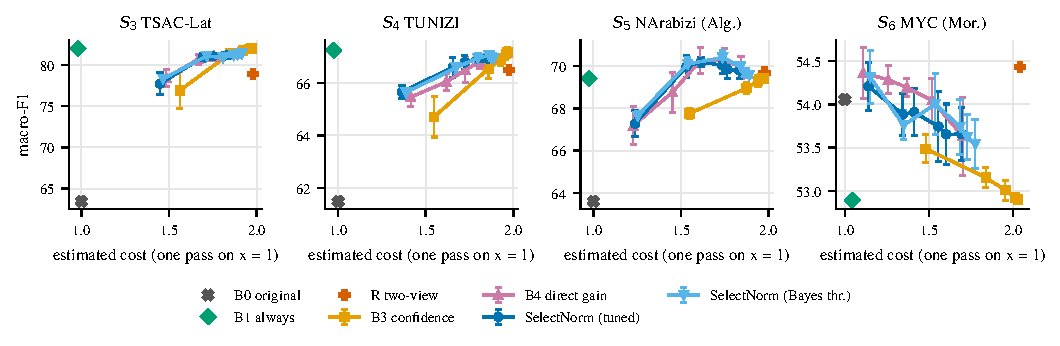
\includegraphics[width=\textwidth]{figures/pareto.pdf}
\caption{Macro-F1 against estimated inference cost (mE5, batch size 1, CPU; one pass of $f$ on $x$ = 1; per-sentence encoder costs from a token-length model fitted to measured latencies, see \cref{app:repro}), for $\lambda\in\{0,.01,.02,.05,.1,.2\}$; error bars: s.d.\ over seeds. Each system is charged for what it runs: B0 one pass on $x$; B1 the normalizer and one pass on $T(x)$; learned routers the first pass and the normalizer (sunk) plus the second pass when selected; B3 the first pass plus normalizer and second pass when selected; R both passes.}
\label{fig:pareto}
\end{figure*}
Each single-view system runs one encoder pass: B0 costs 1.00 and B1 0.97--1.04 passes on $x$ (the normalizer adds about 0.4\%). A router that decides from $p_0$ has already paid for the first pass: at $\lambda=0$, SelectNorm-adapt costs 1.69--1.88 passes for mE5 and 1.43--1.88 across encoders, against 1.89--2.05 for the two-view ensemble. Raising $\lambda$ lowers the cost (to 1.14--1.45 for mE5 at $\lambda=0.2$), but macro-F1 falls towards that of B0 (\cref{fig:pareto}). Per-input routing of this kind is thus never cheaper than the better single view and, never being relevantly more accurate (at most $+0.6$ points, not significant), offers no accuracy--cost advantage over it; it saves compute only relative to running both views. Thresholding with each input's own avoidable cost instead of the mean only moves points along the same frontier. These costs are token-model estimates; running the deployed pipeline end to end, with live routing decisions that reproduce the archived ones exactly, gives the same picture (B1 0.91--1.05, SelectNorm-adapt 1.31--1.97, R 1.91--2.07 passes; \cref{app:repro}). Descriptively, B4 and B3 trace similar curves, and the untuned Bayes threshold a curve close to that of tuned thresholds.

\subsection{Where per-input routing fails (RQ5)}
\label{sec:mechanism}
\begin{table*}[t]
\centering\footnotesize\setlength{\tabcolsep}{3.2pt}
\resizebox{\textwidth}{!}{\begin{tabular}{@{}llrrrrrrrrrr@{}}\toprule
 & & \multicolumn{2}{c}{(M1) disagreement} & \multicolumn{4}{c}{(M2) direction} & \multicolumn{2}{c}{(M3) benefit} & \multicolumn{2}{c}{(M4) headroom}\\
\cmidrule(lr){3-4}\cmidrule(lr){5-8}\cmidrule(lr){9-10}\cmidrule(lr){11-12}
Enc. & Set & $P(D)$ & AUC$_\pi$ & $P(W|D)$ & AUC$_\rho$ & AUC$_\rho^{\rm tgt}$ & gap & $\Delta_{\rm src}$ & $\Delta_{\rm tgt}$ & oracle & vs.\ ref.\\\midrule
mE5 & $S_3$ & 34 & 0.68 & 77 & 0.66 & 0.64 & +3 & -0.6$^{*}$ & +0.0 & 8.0 & -0.3\\
 & $S_4$ & 33 & 0.64 & 57 & 0.56 & 0.58 & +19$^{*}$ & -0.3 & -0.1 & 14.1 & +4.6\\
 & $S_5$ & 29 & 0.62 & 58 & 0.63 & 0.57$^\circ$ & +15$^{*}$ & +0.2 & +0.7 & 12.4 & +3.2\\
 & $S_6$ & 21 & 0.74 & 47 & 0.54 & 0.56 & +20$^{*}$ & -0.5 & +0.2 & 9.7 & +4.6\\
\midrule
XLM-R & $S_3$ & 36 & 0.64 & 72 & 0.71 & 0.68 & +3 & +1.0$^{*}$ & +0.8 & 10.3 & +5.9\\
 & $S_4$ & 31 & 0.66 & 64 & 0.57 & 0.57 & +11$^{*}$ & -0.5 & +0.3 & 10.7 & +7.6\\
 & $S_5$ & 23 & 0.69 & 69 & 0.45$^\circ$ & 0.60$^\circ$ & +11$^{*}$ & +0.3 & -0.7 & 7.3 & +2.1\\
 & $S_6$ & 28 & 0.72 & 69 & 0.44 & 0.66 & -8$^{*}$ & -3.3$^{*}$ & +1.1$^{*}$ & 9.8 & +4.5\\
\midrule
LaBSE & $S_3$ & 30 & 0.69 & 73 & 0.61 & 0.53$^\circ$ & -0 & +0.1 & -0.1 & 7.9 & +1.3\\
 & $S_4$ & 34 & 0.65 & 62 & 0.57 & 0.59 & +6$^{*}$ & -0.4 & -0.4 & 13.0 & +5.7\\
 & $S_5$ & 34 & 0.65 & 58 & 0.59 & 0.55$^\circ$ & +3 & +0.4 & +0.2 & 14.9 & +7.5\\
 & $S_6$ & 31 & 0.68 & 33 & 0.57 & 0.64 & +16$^{*}$ & -2.6$^{*}$ & +0.8$^{*}$ & 11.8 & +5.3\\
\midrule
MARBERTv2 & $S_3$ & 39 & 0.69 & 70 & 0.63 & 0.60 & +1 & +0.1 & -0.3 & 11.5 & +0.8\\
 & $S_4$ & 37 & 0.71 & 60 & 0.61 & 0.64 & +13$^{*}$ & +0.4 & +2.8$^{*}$ & 16.5 & +2.0\\
 & $S_5$ & 31 & 0.73 & 57 & 0.63 & 0.54$^\circ$ & +13$^{*}$ & +0.2 & +1.1 & 15.3 & +3.6\\
 & $S_6$ & 30 & 0.71 & 59 & 0.55 & 0.63 & +4$^{*}$ & -0.3 & +1.1$^{*}$ & 12.1 & -0.7\\
\bottomrule\end{tabular}
}
\caption{The four mechanisms of \cref{sec:formulation} ($T_{\rm cons}$, Arabic-script classifier, mean of five seeds). (M1) disagreement rate (\%) and AUC of label-free, target-cross-fitted $\hat\pi$. (M2) win rate of $T(x)$ on disagreements (\%), AUC of source-trained $\hat\rho$, AUC of a diagnostic $\hat\rho$ cross-validated on target labels (not deployable), and calibration gap of source $\hat\rho$ (points). (M3) macro-F1 gain over the best single view of the rule $\hat\rho>\nicefrac12$ with source and with target-CV $\hat\rho$. (M4) oracle headroom over the best view, and the same minus the headroom between two bootstrap-resampled classifiers on the same input (a diagnostic reference, not a decomposition; see \cref{tab:noise}). $^\circ$: the 95\% interval of the AUC contains 0.5; $^{*}$: the interval of the gap or gain excludes 0 (1{,}000 seed-averaged bootstrap resamples; all intervals in \cref{tab:mechanism-ci}). Test labels are used for analysis only.}
\label{tab:mechanism}
\end{table*}
The factorization lets us measure each sub-problem separately (\cref{tab:mechanism}).

\paragraph{(M1) Disagreement is moderately predictable.} Between 21\% and 39\% of inputs change label under normalization, and the label-free estimate ranks them with AUC 0.62--0.74; every 95\% interval lies between 0.57 and 0.77 (\cref{tab:mechanism-ci}). Re-estimating $\hat\pi$ on unlabeled target text raises this AUC most on MYC (for mE5 from 0.67 with source training to 0.74), but the Bayes rule at $\lambda=0$ depends on $\hat\rho$ alone (\cref{sec:formulation}); accordingly SelectNorm-src and -adapt differ by at most about half a point at $\lambda=0$.

\paragraph{(M2) Direction is weakly predictable from $z$, even in domain.} Which view is right when they disagree is ranked by source-trained $\hat\rho$ with AUC 0.54--0.71 in 14 of 16 cells (interval upper bounds at most 0.76); for XLM-R on Algerian text the interval includes 0.5, and on Moroccan text it lies below it ($[0.41,0.48]$). Fitting $\hat\rho$ on target labels by cross-validation, an upper reference that no deployable system has, reaches 0.53--0.68 (upper bounds at most 0.73), and its interval includes 0.5 in five cells. With linear estimators, the decision-point features thus carry little information about direction in any domain we tested; this does not exclude that other features or estimators would predict it better. What does change across domains is the \emph{level} of $\rho$: the win rate ranges from 33\% to 77\% across encoder--set pairs, and source $\hat\rho$ is miscalibrated out of domain, with gaps whose intervals exclude zero in 11 of 12 out-of-domain cells (up to $+20$ points).

\paragraph{(M3) The expected benefit follows.} The rule $\hat\rho>\nicefrac12$ gains between $-3.3$ and $+1.0$ points over the best single view with source estimates; only one gain has an interval above zero (XLM-R, $S_3$, $+1.0$), and three losses lie below zero. With the target-CV ceiling the change is $-0.7$ to $+2.8$, with interval upper bounds of at most $+3.9$. Most of the gap between routing and the oracle is therefore not a transfer problem: with these features and a linear estimator, it remains when the router is fitted on the target.

\paragraph{(M4) A reference for the oracle headroom.} The oracle gains 7--17 points over the best view, which looks like large headroom. Two classifiers that differ only in a bootstrap resample of their training data, applied to the same input, show 3--15 points of the same kind of headroom without any normalization. This reference is a diagnostic, not a decomposition: it depends strongly on how the two classifiers are made (2--6 points with 80\% subsamples, 5--22 points with weaker regularization; \cref{tab:noise}), so it cannot say how much of the views' headroom is recoverable. It does show that oracle headroom of this size arises from training-sample variability alone, and that oracle headroom is a weak indicator of what a router can gain.

\paragraph{Linguistic conditions.} On the Tunisian and Algerian sets, always normalizing helps less on inputs with many French or English tokens or low lexicon coverage, for every encoder but one case (XLM-R, TUNIZI, French/English) (\cref{tab:taxonomy}); negation and length show no consistent pattern. On MYC the net effect of every condition has a different sign for different encoders, so the main determinant of whether normalization pays there is the encoder--dialect pair, not a property of the input that $z$ could observe.

\begin{table*}[t]
\centering\footnotesize\setlength{\tabcolsep}{4pt}
\begin{tabular}{@{}lrrrr@{}}\toprule
Condition (share of $S_3$/$S_4$/$S_5$/$S_6$) & $S_3$ & $S_4$ & $S_5$ & $S_6$\\\midrule
French/English $\ge$30\% (9/12/12/22) & +4.3 \scriptsize[+0,+11] & +4.3 \scriptsize[-2,+13] & +1.6 \scriptsize[-3,+5] & -0.1 \scriptsize[-9,+7]\\
not French/English $\ge$30\% (91/88/88/78) & +17.0 \scriptsize[+15,+20] & +7.6 \scriptsize[+5,+9] & +6.5 \scriptsize[+5,+10] & +1.3 \scriptsize[-11,+12]\\
negation rule applied (8/12/26/6) & +14.0 \scriptsize[+6,+18] & +5.9 \scriptsize[-4,+20] & +4.0 \scriptsize[-4,+9] & +2.1 \scriptsize[-9,+15]\\
not negation rule applied (92/88/74/94) & +16.1 \scriptsize[+14,+18] & +7.4 \scriptsize[+6,+11] & +6.5 \scriptsize[+3,+11] & +1.0 \scriptsize[-11,+10]\\
lexicon coverage $<$50\% (51/57/81/85) & +12.3 \scriptsize[+11,+14] & +4.5 \scriptsize[+2,+9] & +3.7 \scriptsize[+1,+6] & +0.8 \scriptsize[-11,+11]\\
not lexicon coverage $<$50\% (49/43/19/15) & +19.7 \scriptsize[+17,+23] & +10.8 \scriptsize[+9,+14] & +15.1 \scriptsize[+8,+22] & +2.4 \scriptsize[-11,+13]\\
$\le$3 tokens (42/28/2/27) & +14.2 \scriptsize[+10,+16] & +8.4 \scriptsize[+0,+15] & +13.2 \scriptsize[-18,+35] & +0.7 \scriptsize[-10,+10]\\
not $\le$3 tokens (58/72/98/73) & +17.2 \scriptsize[+13,+20] & +6.8 \scriptsize[+3,+10] & +5.7 \scriptsize[+4,+10] & +1.2 \scriptsize[-11,+11]\\
\bottomrule\end{tabular}

\caption{Net effect of always normalizing (help minus harm per 100 inputs) by input condition, mean over the four encoders, range in brackets. Conditions were fixed before inspection.}
\label{tab:taxonomy}
\end{table*}

\subsection{Few target labels (RQ6)}
\begin{figure*}[t]
\centering
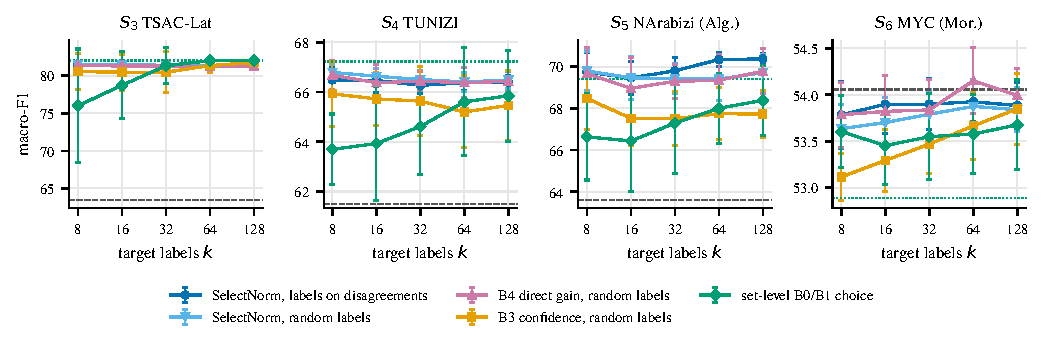
\includegraphics[width=\textwidth]{figures/fewlabel.pdf}
\caption{Few-label adaptation (mE5): macro-F1 against the number $k$ of labelled target sentences (5 draws $\times$ 5 seeds; error bars: s.d.). Dashed: B0; dotted: B1. ``Set-level choice'' picks B0 or B1 by accuracy on the $k$ labels.}
\label{fig:fewlabel}
\end{figure*}
With $k$ labelled target sentences, re-estimating the scalar shift of $\hat\rho$ changes macro-F1 relative to zero-shot SelectNorm-adapt with the same threshold by $-1.4$ to $+1.5$ points across encoders, regimes, sets and $k$ (mean $-0.01$; \cref{fig:fewlabel}). Spending the labels on disagreements, which \cref{prop:efficiency} shows to be $1/P(D{=}1)$ times more informative about the shift, makes little difference: averaged over encoders and sets, SelectNorm with targeted labels is between $-0.1$ and $+0.2$ points from SelectNorm with random labels at every $k$ (descriptive; not tested). In the Arabic-script regime, SelectNorm is clearly better than a set-level choice between B0 and B1 when $k\le 16$ (by 2.6--2.9 points on average), and the advantage shrinks to 0.3 points at $k=128$, consistent with M2: most of the usable signal is set-level.

\subsection{Normalizer, consistency and classifier regime}
\paragraph{Safeguards.} The safeguards of $T_{\rm cons}$ matter more than routing: always normalizing with $T_{\rm lex}$ or $T_{\rm rule}$ instead loses 4--11 points on every set for mE5, and routing over those normalizers recovers only part of the loss (\cref{tab:ablation}). Keeping out-of-lexicon tokens in Latin script ($T_{\rm cov}$) reduces disagreements by about a third and makes routing nearly irrelevant; it is worse than $T_{\rm cons}$ on the Tunisian sets and slightly better on $S_5$ and $S_6$.

\paragraph{Consistency with human transliteration (RQ4).} On NArabizi, B1 agrees with the prediction that $f$ makes on the human Arabic-script version of the same sentence for 73--77\% of inputs, against 61--67\% for B0 and 73--76\% for SelectNorm-adapt, so routing does not increase agreement further; $f$ itself reaches 65--77 macro-F1 on the human transliterations (per-encoder values in the released \texttt{consistency.csv}).

\paragraph{Classifier trained on both scripts.} When $f$ also sees synthetic Latin renderings (\textsc{+syn}, \cref{tab:main-syn}), the original view improves and the two views become more complementary: the oracle headroom stays similar, the win rate on disagreements moves towards 50\%, and SelectNorm-adapt exceeds the better single view in several cells. Against that view it is relevantly better once with Holm correction (MARBERTv2, $S_4$, $+1.1$) and twice more under the protocol's unadjusted criterion (mE5, $S_3$ $+2.1$, $S_4$ $+1.4$), and relevantly worse in two MYC cells under both (LaBSE $-2.4$, MARBERTv2 $-1.8$). Confidence thresholding and the ensemble share the gains; SelectNorm is never significantly better than B4 (worse once, $-0.4$).
